\documentclass{article}

\usepackage[preprint]{neurips_2026}

\usepackage[utf8]{inputenc}
\usepackage[T1]{fontenc}
\usepackage{hyperref}
\usepackage{url}
\usepackage{booktabs}
\usepackage{amsmath,amsfonts}
\usepackage{nicefrac}
\usepackage{microtype}
\usepackage{xcolor}
\usepackage{graphicx}

\newcommand{\norm}[1]{\lVert #1 \rVert}
\newcommand{\fp}{\texttt{fp32}}
\newcommand{\ieight}{\texttt{int8}}
\newcommand{\ifour}{\texttt{int4}}

\title{Does quantization make a network easier to fool?}

\author{%
  Nayan Patel \\
  ESE 5420 final project (early draft)\\
  University of Pennsylvania
}

\begin{document}

\maketitle

\begin{abstract}
Networks are routinely quantized before deployment, but their robustness is rarely re-checked afterwards. We ask: does post-training weight quantization (\ieight{} and \ifour{}) of a two-layer MLP on MNIST raise its Lipschitz bound and lower its accuracy under the fast gradient sign attack (FGSM), and does weight decay protect against any such loss? The course baseline is multinomial logistic regression with an $\ell_2$ penalty tuned by 5-fold cross-validation. It reaches $91.8\%$ validation accuracy under FGSM at $\epsilon = 0.1$. Preliminary results show that weight decay matters far more than quantization: raising it from $0$ to $10^{-2}$ cuts the MLP's spectral-norm bound from $30.2$ to $4.2$ and doubles FGSM accuracy at $\epsilon = 0.1$ ($28.5\%$ to $58.2\%$) at a cost of $4.7$ points of clean accuracy. \ieight{} is indistinguishable from full precision. \ifour{} changes the bound by under $2\%$; it lowers FGSM accuracy by two to three points only for unregularized models at small $\epsilon$, and appears to \emph{raise} it for weight-decayed models at larger $\epsilon$, a pattern that needs a stronger attack before it can be believed. The test set is untouched. This draft lists the experiments still to run.
\end{abstract}

\section{Introduction}

\paragraph{Question.} A classifier is easy to fool if a small change to its input moves its output a long way. Two standard ways to quantify this are the accuracy that survives a gradient-based attack such as FGSM \citep{goodfellow2015explaining}, and the Lipschitz constant of the network, which caps how far the output can move per unit change in the input \citep{fazlyab2019efficient}. Weight decay shrinks the weights, and so the Lipschitz bound, and is expected to make a network harder to fool. This project adds one step that practice adds to almost every deployed model: rounding the trained weights to a few bits. We ask whether post-training weight quantization to \ieight{} or \ifour{} raises the Lipschitz bound and lowers FGSM accuracy of a two-layer MLP on MNIST, and whether weight decay protects against that loss.

\paragraph{Why it matters.} Post-training quantization is the default way to shrink a model for inference, and it is usually validated on clean accuracy alone. Prior work on larger networks reports that quantized models can be more vulnerable to adversarial inputs because rounding error is amplified layer by layer, and proposes controlling the Lipschitz constant as the remedy \citep{lin2019defensive}. If that holds even in the smallest setting, anyone shipping a small quantized model should re-check robustness; if plain weight decay removes the effect, the fix is nearly free. A precisely measured null is also useful: it would say that for small networks the robustness budget is set at training time, not at quantization time.

\paragraph{What we compare.} The baseline is multinomial logistic regression with an $\ell_2$ penalty, a course method whose logits have a Lipschitz constant \emph{exactly} equal to the spectral norm of its weight matrix. We compare it with two-layer MLPs trained at four weight-decay values. Every trained model is evaluated at three precisions (\fp{}, \ieight{}, \ifour{}), giving a $(1 + 4) \times 3$ grid of settings. For each we report clean accuracy, FGSM accuracy at three attack sizes, and Lipschitz bounds. The key figure plots FGSM accuracy against the Lipschitz upper bound. This is an early draft: results are preliminary and on the validation split, and Section~\ref{sec:remaining} lists what remains.


\section{Data}
\label{sec:data}

\paragraph{Source.} We use MNIST: \url{http://yann.lecun.com/exdb/mnist/}, loaded through \texttt{torchvision.datasets.MNIST}. It is distributed under the Creative Commons Attribution-ShareAlike 3.0 licence. It holds $70{,}000$ grayscale images of handwritten digits, $28 \times 28$ pixels each, in a fixed split of $60{,}000$ training and $10{,}000$ test images. Each input is flattened to $d = 784$ pixel values and the output is one of 10 digit classes. No rows were dropped.

\paragraph{Preprocessing.} Pixels are divided by 255 so that inputs lie in $[0,1]^{784}$. We do not standardize. This keeps the attack size $\epsilon$ in raw pixel units, and it means no statistic is learned from the data before splitting.

\paragraph{Split.} The $60{,}000$ training images are permuted once (seed 0) and divided into $50{,}000$ training and $10{,}000$ validation images. Class counts range from $4{,}485$ to $5{,}635$ in the training part and from $936$ to $1{,}107$ in the validation part. All model fitting and cross-validation use only the $50{,}000$; every number in this draft is measured on the $10{,}000$ validation images. The $10{,}000$ MNIST test images have not been loaded by any script and will be scored once, after every choice is fixed (Section~\ref{sec:remaining}).

\section{Method}
\label{sec:method}

\subsection{Baseline: multinomial logistic regression}

The baseline is $f(x) = Wx + b$ with $W \in \mathbb{R}^{10 \times 784}$, trained with the softmax cross-entropy loss and an $\ell_2$ penalty on $W$, using scikit-learn's L-BFGS solver. The penalty is set by $C = 1/\lambda$, the inverse regularization strength.

\paragraph{Tuning.} $C$ is chosen from $\{10^{-4}, 10^{-3}, 10^{-2}, 10^{-1}, 1, 10, 10^{2}\}$ by stratified 5-fold cross-validation inside the $50{,}000$ training images, selecting the value with the highest mean fold accuracy. The procedure is repeated with three fold-shuffle seeds (0, 1, 2). The model is then refit on all $50{,}000$ images at the chosen $C$. Table~\ref{tab:cv} gives the cross-validation scores.

\subsection{Comparison: two-layer MLP with weight decay}

The comparison model is $f(x) = W_2\,\mathrm{ReLU}(W_1 x + b_1) + b_2$ with 256 hidden units, implemented in PyTorch. It is trained with SGD (momentum $0.9$, learning rate $0.05$, batch size 128, 15 epochs) on the cross-entropy loss. Weight decay $\lambda \in \{0, 10^{-4}, 10^{-3}, 10^{-2}\}$ is applied to all parameters as a coupled $\ell_2$ penalty. Each setting is trained with seeds 0, 1 and 2, which set the initialization and the minibatch order.

\paragraph{Tuning.} Weight decay is the variable under study, so all four values are reported rather than one being selected. The rest of the recipe was fixed before any result was seen and has not been tuned. For the final test-set evaluation, one weight decay will be selected on the validation split with a rule stated in advance (Section~\ref{sec:remaining}).

\subsection{Post-training weight quantization}

Each trained weight matrix $W$ is quantized on its own (per-tensor), symmetrically, to $b$ bits. With $q = 2^{b-1} - 1$ and scale $s = \max_{ij} |W_{ij}| / q$,
\begin{equation}
  Q_b(W) = s \cdot \mathrm{clip}\bigl(\mathrm{round}(W / s),\, -q,\, q\bigr),
\end{equation}
so \ieight{} uses $q = 127$ and \ifour{} uses $q = 7$ (15 levels). Only weights are quantized. Biases and activations stay in 32-bit floating point, so the quantized model is an ordinary differentiable network with rounded weights; its input gradients are exact. Rounding activations as well would make input gradients vanish almost everywhere and FGSM would report false robustness. The same procedure is applied to the logistic regression weights.

\subsection{Lipschitz bounds}

\paragraph{Upper bound.} Because ReLU is 1-Lipschitz, the MLP's logits satisfy $\norm{f(x) - f(x')}_2 \le \norm{W_2}_2 \norm{W_1}_2 \norm{x - x'}_2$, where $\norm{\cdot}_2$ on a matrix is its spectral norm \citep{fazlyab2019efficient}. We report $\hat{L} = \norm{W_2}_2 \norm{W_1}_2$. For logistic regression the bound is the exact Lipschitz constant, $L = \norm{W}_2$.

\paragraph{Lower bound.} The network is piecewise linear, so the spectral norm of its input Jacobian at any point is a lower bound on the true constant. We report the largest value over the validation images, $\max_i \norm{W_2\,\mathrm{diag}(\mathbf{1}[W_1 x_i + b_1 > 0])\,W_1}_2$. The true constant lies between the two bounds.

\paragraph{What quantization can do to the bound.} Rounding moves each weight by at most $s/2$, so for an $m \times n$ matrix $\bigl|\norm{Q_b(W)}_2 - \norm{W}_2\bigr| \le \norm{Q_b(W) - W}_2 \le \tfrac{s}{2}\sqrt{mn}$. The bound can therefore move in either direction; whether it moves by a meaningful amount is an empirical question.

\subsection{FGSM attack}

For an image $x$ with label $y$ and loss $\ell$, the attack is $x_{\mathrm{adv}} = \mathrm{clip}_{[0,1]}\bigl(x + \epsilon\, \mathrm{sign}(\nabla_x \ell(f(x), y))\bigr)$ \citep{goodfellow2015explaining}. Each model is attacked with its own gradients (white box); a quantized model is attacked through its quantized weights. FGSM perturbations are bounded in $\ell_\infty$, while the Lipschitz bounds are in $\ell_2$; an $\ell_\infty$ perturbation of size $\epsilon$ has $\ell_2$ norm at most $\epsilon\sqrt{d} = 28\epsilon$.

\section{Experimental setup}
\label{sec:setup}

\paragraph{Metrics.} (i) Clean accuracy on the validation split. (ii) FGSM accuracy, the fraction of validation images still classified correctly after the attack, at $\epsilon \in \{0.05, 0.1, 0.2\}$; $\epsilon = 0.1$ is the headline value. (iii) The Lipschitz upper bound for every model and the lower bound for the MLPs.

\paragraph{Validation protocol.} Cross-validation for the baseline is run inside the $50{,}000$ training images only. The validation split is used for reporting and, later, for selecting the MLP's weight decay. No preprocessing step is fit to data. The test set is used once, at the end.

\paragraph{Error bars.} \emph{Baseline.} Logistic regression is a convex problem and all three cross-validation repeats selected the same $C$, so its three runs are identical and there is no seed spread. Its error bar is a percentile bootstrap: the $10{,}000$ validation images are resampled with replacement $2{,}000$ times, and we report the $2.5$th and $97.5$th percentiles of the resampled accuracy. \emph{MLPs.} We report the mean and sample standard deviation over three seeds. The sampling error of the validation set itself is at most $0.5$ percentage points (binomial standard error at $n = 10{,}000$). \emph{Quantization effects.} A quantized model and its \fp{} parent are the same trained network, so we also report the per-seed difference (\ifour{} minus \fp{}) and its standard deviation over seeds. A difference smaller than its spread is called a tie.

\paragraph{Reproducibility.} Code and saved results are at \url{https://github.com/nayanp38/ESE5420_final_project}. All seeds are fixed; the tables and figures in this draft are generated from the saved result files by a script.

\section{Preliminary results}
\label{sec:results}

All numbers in this section are on the validation split.

\subsection{Baseline}

\begin{table}[t]
  \caption{Tuning the baseline. Mean stratified 5-fold cross-validation accuracy of logistic regression inside the $50{,}000$ training images, averaged over three fold-shuffle seeds; the fold standard error is the standard deviation over the five folds divided by $\sqrt{5}$. $C = 0.1$ is selected in every repeat; $C = 1$ is within about one standard error of it.}
  \label{tab:cv}
  \centering
  \small
  \begin{tabular}{lccccccc}
\toprule
$C = 1/\lambda$ & $10^{-4}$ & $10^{-3}$ & $10^{-2}$ & $10^{-1}$ & $10^{0}$ & $10^{1}$ & $10^{2}$ \\
\midrule
CV accuracy (\%) & 83.75 & 88.77 & 91.15 & \textbf{92.09} & 91.95 & 91.35 & 90.99 \\
Fold SE (points) & 0.16 & 0.16 & 0.13 & 0.13 & 0.13 & 0.15 & 0.14 \\
\bottomrule
\end{tabular}

\end{table}

\begin{table}[t]
  \caption{Baseline result. Logistic regression ($C = 0.1$) on the $10{,}000$ validation images, at three weight precisions. Brackets are 95\% bootstrap intervals ($2{,}000$ resamples of the validation images). $L$ is the exact Lipschitz constant of the logits (spectral norm of the weights). \ieight{} matches \fp{}; \ifour{} costs about half a point of clean accuracy and two points of FGSM accuracy at $\epsilon = 0.05$.}
  \label{tab:baseline}
  \centering
  \small
  \begin{tabular}{llllll}
\toprule
 & & \multicolumn{3}{c}{FGSM accuracy (\%)} & \\
\cmidrule(lr){3-5}
Weights & Clean accuracy (\%) & $\epsilon = 0.05$ & $\epsilon = 0.1$ & $\epsilon = 0.2$ & $L$ \\
\midrule
fp32 & 91.8 [91.3, 92.3] & 49.2 [48.2, 50.2] & 6.6 [6.2, 7.1] & 0.0 [0.0, 0.0] & 7.57 \\
int8 & 91.8 [91.3, 92.3] & 49.1 [48.1, 50.0] & 6.6 [6.1, 7.1] & 0.0 [0.0, 0.0] & 7.58 \\
int4 & 91.3 [90.8, 91.9] & 47.3 [46.3, 48.2] & 5.9 [5.4, 6.4] & 0.0 [0.0, 0.0] & 7.66 \\
\bottomrule
\end{tabular}

\end{table}

Cross-validation selected $C = 0.1$ in all three repeats (Table~\ref{tab:cv}). The margin over $C = 1$ is $0.14$ points, about one fold standard error, so the two are a tie in cross-validation; we keep $C = 0.1$ because the selection rule was fixed in advance. Refit on the full training split, the baseline reaches $91.8\%$ clean accuracy, 95\% interval $[91.3, 92.3]$ (Table~\ref{tab:baseline}). It is very fragile: FGSM accuracy is $49.2\%$ at $\epsilon = 0.05$, $6.6\%$ $[6.2, 7.1]$ at $\epsilon = 0.1$, and one image in $10{,}000$ at $\epsilon = 0.2$.

\subsection{Weight decay, the Lipschitz bound and FGSM accuracy}

\begin{table}[t]
  \caption{MLP results on the validation split, mean $\pm$ standard deviation over three seeds. Weight decay lowers both Lipschitz bounds and raises FGSM accuracy at $\epsilon = 0.1$; \ieight{} rows match their \fp{} rows; \ifour{} rows differ by a few points in FGSM accuracy, in a direction that depends on weight decay.}
  \label{tab:mlp}
  \centering
  \footnotesize
  \setlength{\tabcolsep}{4pt}
  \begin{tabular}{llcccccc}
\toprule
 & & & \multicolumn{3}{c}{FGSM accuracy (\%)} & \multicolumn{2}{c}{Lipschitz bounds} \\
\cmidrule(lr){4-6} \cmidrule(lr){7-8}
Weight decay & Weights & Clean (\%) & $\epsilon = 0.05$ & $\epsilon = 0.1$ & $\epsilon = 0.2$ & Upper & Lower \\
\midrule
0 & fp32 & 97.7 $\pm$ 0.1 & 79.2 $\pm$ 0.7 & 28.5 $\pm$ 0.6 & 5.1 $\pm$ 0.4 & 30.17 $\pm$ 0.53 & 16.71 $\pm$ 0.90 \\
 & int8 & 97.7 $\pm$ 0.1 & 79.0 $\pm$ 0.7 & 28.5 $\pm$ 0.6 & 5.1 $\pm$ 0.4 & 30.18 $\pm$ 0.53 & 16.72 $\pm$ 0.90 \\
 & int4 & 97.4 $\pm$ 0.2 & 76.2 $\pm$ 0.5 & 26.9 $\pm$ 2.4 & 4.9 $\pm$ 0.0 & 30.61 $\pm$ 0.38 & 16.77 $\pm$ 0.34 \\
\addlinespace
$10^{-4}$ & fp32 & 97.7 $\pm$ 0.0 & 81.4 $\pm$ 0.9 & 32.1 $\pm$ 1.4 & 2.1 $\pm$ 0.4 & 24.06 $\pm$ 0.42 & 13.37 $\pm$ 0.46 \\
 & int8 & 97.7 $\pm$ 0.0 & 81.4 $\pm$ 0.8 & 32.1 $\pm$ 1.3 & 2.1 $\pm$ 0.4 & 24.06 $\pm$ 0.42 & 13.34 $\pm$ 0.48 \\
 & int4 & 97.3 $\pm$ 0.2 & 80.9 $\pm$ 1.3 & 34.4 $\pm$ 1.5 & 2.3 $\pm$ 0.2 & 24.38 $\pm$ 0.31 & 13.48 $\pm$ 0.31 \\
\addlinespace
$10^{-3}$ & fp32 & 97.2 $\pm$ 0.1 & 87.2 $\pm$ 0.1 & 55.9 $\pm$ 3.3 & 4.4 $\pm$ 0.5 & 11.02 $\pm$ 0.10 & 6.40 $\pm$ 0.07 \\
 & int8 & 97.2 $\pm$ 0.2 & 87.2 $\pm$ 0.1 & 55.9 $\pm$ 3.3 & 4.4 $\pm$ 0.5 & 11.02 $\pm$ 0.11 & 6.40 $\pm$ 0.07 \\
 & int4 & 97.0 $\pm$ 0.2 & 87.6 $\pm$ 0.6 & 59.8 $\pm$ 2.7 & 6.3 $\pm$ 0.7 & 11.03 $\pm$ 0.11 & 6.18 $\pm$ 0.08 \\
\addlinespace
$10^{-2}$ & fp32 & 93.0 $\pm$ 0.1 & 81.7 $\pm$ 0.7 & 58.2 $\pm$ 2.9 & 9.4 $\pm$ 1.3 & 4.16 $\pm$ 0.04 & 3.56 $\pm$ 0.02 \\
 & int8 & 93.0 $\pm$ 0.1 & 81.8 $\pm$ 0.7 & 58.2 $\pm$ 2.9 & 9.4 $\pm$ 1.3 & 4.16 $\pm$ 0.04 & 3.56 $\pm$ 0.02 \\
 & int4 & 92.6 $\pm$ 0.2 & 81.5 $\pm$ 0.4 & 59.9 $\pm$ 2.0 & 11.8 $\pm$ 1.3 & 4.12 $\pm$ 0.05 & 3.47 $\pm$ 0.01 \\
\bottomrule
\end{tabular}

\end{table}

\begin{figure}[t]
  \centering
  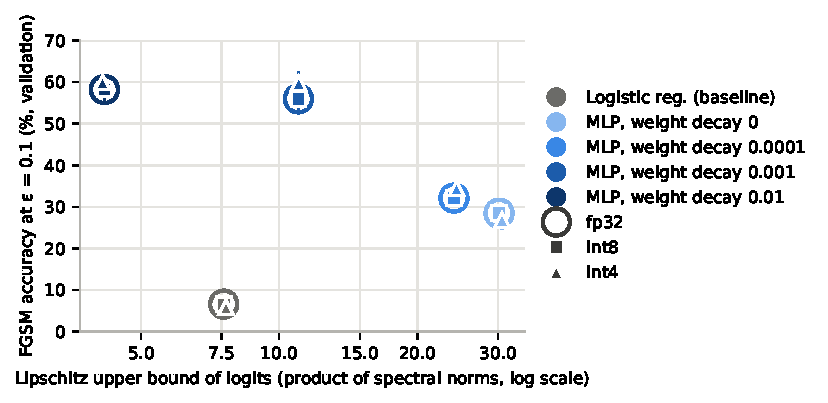
\includegraphics[width=\linewidth]{figures/key_figure.pdf}
  \caption{Key figure (first version). FGSM accuracy at $\epsilon = 0.1$ against the Lipschitz upper bound, on the validation split. Points are means over three seeds and bars are $\pm 1$ standard deviation; the baseline has no seed spread. Within the MLP family a smaller bound goes with higher robust accuracy, and the three precisions of each model sit almost on top of each other. The bound does not rank models across families: logistic regression has a small bound and the lowest robust accuracy.}
  \label{fig:key}
\end{figure}

Weight decay does what the Lipschitz argument predicts (Table~\ref{tab:mlp}, Figure~\ref{fig:key}). Going from $\lambda = 0$ to $10^{-2}$ lowers the upper bound from $30.2 \pm 0.5$ to $4.2 \pm 0.04$ and the lower bound from $16.7 \pm 0.9$ to $3.6 \pm 0.02$. The old lower bound is about four times the new upper bound, so the true constant falls by at least that factor. FGSM accuracy at $\epsilon = 0.1$ rises from $28.5 \pm 0.6\%$ to $58.2 \pm 2.9\%$. The price is clean accuracy, which falls from $97.7\%$ to $93.0\%$. The two largest weight decays are a tie at $\epsilon = 0.1$ ($55.9 \pm 3.3\%$ against $58.2 \pm 2.9\%$), and which is better depends on the attack size: $\lambda = 10^{-3}$ is best at $\epsilon = 0.05$ ($87.2 \pm 0.1\%$) and $\lambda = 10^{-2}$ is best at $\epsilon = 0.2$ ($9.4 \pm 1.3\%$).

The bound orders the MLPs but not the two model families. Logistic regression has $L = 7.6$, below even the \emph{lower} bound of the two least-regularized MLPs, yet its FGSM accuracy at $\epsilon = 0.1$ is $6.6\%$, below all four. A Lipschitz constant limits how fast the logits can move; whether a prediction flips also depends on the margin between the top two logits, which the bound does not see.

\subsection{Quantization}

\begin{figure}[t]
  \centering
  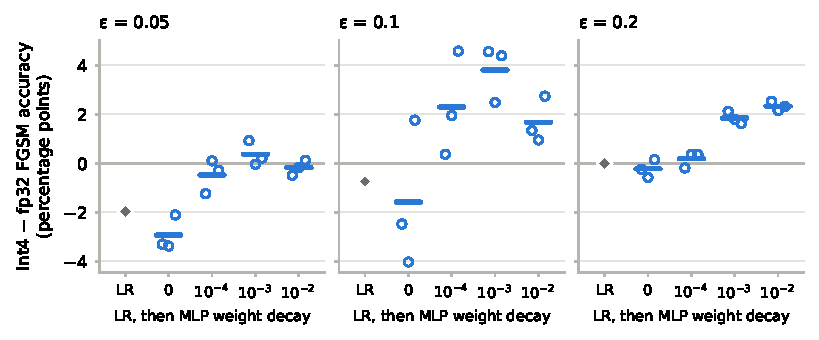
\includegraphics[width=\linewidth]{figures/int4_minus_fp32.pdf}
  \caption{Effect of \ifour{} quantization on FGSM accuracy: \ifour{} minus \fp{}, in percentage points, on the validation split. Circles are individual seeds (the same trained network before and after rounding), bars are their means, and the diamond is the baseline (one deterministic model). \ifour{} hurts the unregularized models at $\epsilon = 0.05$ and appears to help the weight-decayed MLPs at larger $\epsilon$.}
  \label{fig:diff}
\end{figure}

\paragraph{\ieight{} changes nothing measurable.} Across every model, seed and attack size, the mean \ieight{} minus \fp{} difference in clean or FGSM accuracy is at most $0.15$ points in absolute value, and the upper bound moves by at most $0.02$.

\paragraph{\ifour{} barely moves the bound.} The upper bound changes by $+1.5\%$, $+1.4\%$, $+0.1\%$ and $-0.9\%$ for the four weight decays in increasing order, and by $+1.1\%$ for logistic regression. The first half of the question therefore has a preliminary answer: quantization does not raise the Lipschitz bound by a meaningful amount in this setting.

\paragraph{\ifour{} costs a little clean accuracy.} The loss is $0.2$ to $0.4$ points for the MLPs, consistent in sign across all twelve trained networks, and $0.5$ points for logistic regression.

\paragraph{The effect of \ifour{} on FGSM accuracy depends on weight decay.} Figure~\ref{fig:diff} shows the per-seed differences. At $\epsilon = 0.05$, \ifour{} lowers FGSM accuracy of the unregularized MLP by $2.9 \pm 0.7$ points (all three seeds negative) and of logistic regression by $2.0$ points; with any weight decay the difference is a tie ($-0.5 \pm 0.7$, $+0.4 \pm 0.5$, $-0.2 \pm 0.3$). Read alone, this supports the hypothesis that weight decay protects against quantization. At $\epsilon = 0.1$ and $0.2$, however, \ifour{} networks with $\lambda \ge 10^{-3}$ score \emph{higher} than their \fp{} parents: $+3.8 \pm 1.2$ and $+1.7 \pm 0.9$ points at $\epsilon = 0.1$, and $+1.9 \pm 0.3$ and $+2.3 \pm 0.2$ at $\epsilon = 0.2$, positive in every seed. For the unregularized MLP at $\epsilon = 0.1$ the difference is a tie ($-1.6 \pm 3.0$).

\paragraph{Caveats.} We do not yet believe the apparent gain. FGSM takes a single gradient step, and a model can look robust to it because its gradients are less useful, not because it is harder to fool \citep{athalye2018obfuscated}. Coarse rounding makes many small weights exactly zero, which could produce either a real, slight smoothing (the Jacobian lower bound does fall under \ifour{} for $\lambda \ge 10^{-3}$, from $6.40$ to $6.18$ and from $3.56$ to $3.47$) or a one-step artifact. Three seeds also give a poor estimate of the spread. The stronger attack and the paired analysis in Section~\ref{sec:remaining} are designed to settle this.

\section{Remaining work}
\label{sec:remaining}

\subsection{Experiments to run before Analysis Complete (30 November)}

\begin{enumerate}
  \item \textbf{Paired bootstrap of \ifour{} minus \fp{}.} Save per-image correctness and resample images once for both models, so the interval is on the difference itself. We will state in advance the size of effect that counts (proposed: one percentage point), so that a null result can be reported as ``no loss larger than this''.
  \item \textbf{A stronger attack (PGD).} Repeat the robustness evaluation with projected gradient descent \citep{madry2018towards} at the same $\epsilon$ values. If the \ifour{} gain survives it is real; if it disappears it was an artifact of the one-step attack.
  \item \textbf{Per-row \ifour{} quantization.} Give each output unit its own scale. Same number of bits, smaller rounding error; this separates ``four bits'' from ``this rounding scheme'' and tests whether zeroed small weights drive the \ifour{} effect.
  \item \textbf{Accuracy against attack size.} Extend the three attack sizes already measured to a finer grid and plot accuracy against $\epsilon$ for each setting.
  \item \textbf{Select weight decay and score the test set once.} Choose one weight decay on the validation split with a rule fixed beforehand (proposed: the highest FGSM accuracy at $\epsilon = 0.1$ among settings within one point of the best clean accuracy), then report every final number on the $10{,}000$ test images, once.
  \item \textbf{If time allows.} Five seeds instead of three; logit-margin distributions, to explain why the bound fails across model families; Fashion-MNIST.
\end{enumerate}

\subsection{Outline of the remaining sections}

\begin{itemize}
  \item \textbf{Results (final).} Table~\ref{tab:mlp} and Figure~\ref{fig:key} redone on the test set, with the baseline in every table; paired intervals for each quantization effect; FGSM and PGD side by side; accuracy-against-$\epsilon$ curves.
  \item \textbf{Discussion.} Why weight decay dominates quantization; why the bound ranks models within a family but not across families; how tight the bound is.
  \item \textbf{Limitations.} One small architecture and one easy dataset; a cheap bound, not a tight one such as LipSDP \citep{fazlyab2019efficient}; weight-only post-training quantization; attacks, not certificates.
  \item \textbf{Conclusion.} A direct answer to the title question, with effect sizes and intervals.
\end{itemize}

\bibliographystyle{plainnat}
\bibliography{references}

\end{document}
